\documentclass[preprint,12pt]{elsarticle}

\usepackage{amsmath,amssymb}
\usepackage{booktabs}
\usepackage{graphicx}
\usepackage{hyperref}
\usepackage{url}
\usepackage{xcolor}

\graphicspath{{figures/}}
\hypersetup{colorlinks=true,linkcolor=black,citecolor=blue,urlcolor=blue}

\journal{Journal of Systems Architecture}

\newcommand{\AI}{\mathrm{AI}}

\begin{document}

\begin{frontmatter}

\title{Shape-Conditioned Intensity Classification for Dual-Plan Fusion in DNN Compilers}

\author[inst]{Happy Super}
\ead{happy.super@example.com}

\affiliation[inst]{op={},organization={Affiliation TBD}}

\begin{abstract}
Whether a tensor operator is compute-bound or memory-bound depends on its shape, its dtype, and which intermediates touch off-chip memory.
On a cold-HBM accounting, a width-4096 FP16 GEMM moves from about one FLOP per byte at a single decode row to 1024 FLOP/byte at a 2048-row prefill.
An IO-aware attention plan moves with sequence length.
A plan that writes the score matrix does not.
A fusion bit frozen by operator kind cannot follow those crossings.

We describe a shape-conditioned intensity classifier (SCIC) that labels each producer--consumer site against a datasheet Roofline ridge, and a dual-plan selector that emits a memory-oriented plan (MemMode), a compute-oriented plan (ComputeMode), or both inside a band around the ridge.
The executable prototype binds those plans to stock PyTorch paths.
For MatMul+RMSNorm, a few-shot wall-clock probe chooses between the compiled chain and the eager chain.
For attention, every regime calls PyTorch SDPA, and the epilogue policy compiles that operator together with RMSNorm.

On an idle NVIDIA A40 the GEMM probe matches the faster of the two paths on all seven shapes.
It raises the geometric-mean speedup versus eager from $0.921\times$, the datasheet primary, to $1.055\times$.
The datasheet primary agrees with the probe on one shape.
The attention policy is $1.43\times$ geometric mean against a score-materializing eager baseline, and on this run it is slower than eager library SDPA.
Nsight DRAM counters returned \texttt{ERR\_NVGPUCTRPERM}.
The evaluation reports subgraph wall-clock and logged decisions.
Achieved arithmetic intensity, custom fused kernels, and end-to-end token rate are unmeasured.
\end{abstract}

\begin{highlights}
\item Shape-conditioned intensity labels GEMM and attention before fusion.
\item A wall-clock probe picks the faster GEMM path on all seven A40 shapes.
\item The datasheet primary matches that measured GEMM path on one shape.
\item Compiled SDPA plus norm loses to eager SDPA on five shapes.
\item Evidence is subgraph latency; DRAM performance counters were unavailable.
\end{highlights}

\begin{keyword}
DNN compilers \sep operator fusion \sep Roofline model \sep arithmetic intensity \sep GPU architecture \sep PyTorch
\end{keyword}

\end{frontmatter}

\section{Introduction}
\label{sec:intro}

A fusion compiler that decides from operator adjacency alone is using the wrong feature.
The same matrix product is a different machine regime at decode and at prefill, and the same attention block is a different regime when the score matrix stays on chip than when it is written out.
We treat that fact as a scheduling problem for DNN compilers: classify the site from its shape and its traffic, keep more than one legal plan where the classification is uncertain, and select the executable plan from a measurement when the plans are existing compiler or library paths.

The classifier in this paper is analytical.
Arithmetic intensity is FLOPs divided by a cold off-chip byte count, and the machine ridge is a datasheet peak, not a counter measurement.
The three-way label is a policy band around that ridge.
MemMode fuses the epilogue and prefers the memory side of the band.
ComputeMode keeps the epilogue off the matrix-multiply mainloop and prefers the compute side.
Inside the band the selector emits both plans.
That interface is the systems contribution.
It is the point at which a compiler can refuse a single frozen fusion bit.

The prototype that we time does not lower either plan to a custom kernel.
MemMode and ComputeMode are bound to two PyTorch subgraphs.
On MatMul+RMSNorm, \texttt{always\_fuse} is \texttt{torch.compile} of the chain and \texttt{always\_unfuse} is the eager chain.
A few-shot median picks one of them.
On attention, both sides call PyTorch's \texttt{scaled\_dot\_product\_attention}.
The executable policy, \texttt{compile\_sdpa\_chain}, compiles SDPA together with RMSNorm in every regime, including regimes whose analytical primary would have split the epilogue.
The selected latency copies the median of the chosen baseline.
It does not include a plan-switch cost, because no separate dispatcher is timed.

The idle-GPU archive (\texttt{paper/data/bakeoff\_v4/}, package 0.3.1) is the measurement we quote.
Across seven FP16 MatMul+RMSNorm shapes with $N{=}K{=}4096$, the probe selects the faster path every time, and that choice agrees with the datasheet primary only at $M{=}256$.
The geometric mean moves from $0.921\times$ versus eager, if the datasheet primary is followed, to $1.055\times$ when the probe is followed.
The switch from unfuse to fuse lies between $M{=}256$ and $M{=}512$, inside the ridge band of the A40 datasheet.
Across five attention shapes the library policy is a different result.
It beats a score-materializing eager baseline, and it loses to eager SDPA on every shape and to a split-norm SDPA path on four of the five.
Section~\ref{sec:eval} reports those cells.
It does not convert them into a claim about counter-based intensity.

\paragraph{Contributions}
\begin{enumerate}
\item A shape-conditioned intensity classifier for GEMM, attention prefill and decode, norms, reductions, and ragged grouped GEMM, scored against datasheet ridges for H100 FP16, H100 FP8, A100 FP16, and A40 FP16.
\item A dual-plan rule that emits MemMode, ComputeMode, or both, together with an executable binding of those plans onto PyTorch compile and library SDPA paths, including a few-shot wall-clock probe for every MatMul+RMSNorm shape.
\item An idle-A40 evaluation of that binding against eager, \texttt{torch.compile}, max-autotune, always-fuse, and always-unfuse, with the gap to the faster of fuse and unfuse stated per shape.
\end{enumerate}

\paragraph{Outside this paper}
The artifact emits no custom CUDA kernel for either plan, no Stage-Stream schedule~\cite{Mu2026ComFuse}, and no FlashAttention-3 kernel~\cite{Shah2024FlashAttention3}.
The logged accuracy flag is false on every row.
End-to-end tokens per second are not measured.
A torch-profiler byte count from an earlier A40 package is not used as accuracy.

\section{Background}
\label{sec:background}

\subsection{Roofline as a classifier feature}
\label{sec:roofline}

Williams, Waterman, and Patterson define arithmetic intensity and the machine ridge~\cite{Williams2009Roofline}
\begin{equation}
  \AI = \frac{\mathrm{FLOPs}}{\mathrm{bytes}}, \qquad
  R = \frac{\mathrm{peak\ FLOP/s}}{\mathrm{peak\ byte/s}}.
  \label{eq:roofline}
\end{equation}
A kernel with $\AI < R$ is bandwidth-limited on the classical Roofline.
A kernel with $\AI > R$ is compute-limited.
With no cache reuse, no launch cost, and no overlap, time is $\max(\mathrm{FLOPs}/P,\ \mathrm{bytes}/B)$.
We use this model as a feature that a fusion planner can query.
We do not use it as a latency predictor.
The peaks in Table~\ref{tab:ridges} are public dense Tensor-Core numbers with structural sparsity left unused.
None of them was measured on the A40 that produced Section~\ref{sec:eval}.

\begin{table}[t]
  \centering
  \caption{Datasheet anchors used by SCIC.
  $R$ is peak FLOP/s divided by peak byte/s.
  $M(0.5R)$, $M^{\star}$, and $M(2R)$ are the closed-form row counts at which a square projection $N{=}K{=}4096$ has $\AI$ equal to $0.5R$, $R$, and $2R$.
  The FP8 row uses one-byte elements and the FP8 peak.
  The evaluation machine flag is A40 FP16.}
  \label{tab:ridges}
  \footnotesize
  \setlength{\tabcolsep}{4pt}
  \begin{tabular}{@{}lrrrrrr@{}}
    \toprule
    Anchor & Peak & Memory & $R$ & $M(0.5R)$ & $M^{\star}$ & $M(2R)$ \\
           & (TFLOP/s) & & (FLOP/byte) & & & \\
    \midrule
    H100 SXM FP16 & 989 & 3.35 TB/s & 295.22 & 159.1 & 344.9 & 829.6 \\
    H100 SXM FP8  & 1979 & 3.35 TB/s & 590.75 & 159.2 & 345.2 & 830.2 \\
    A100 80GB FP16 & 312 & 2.039 TB/s & 153.02 & 79.5 & 165.4 & 359.8 \\
    A40 FP16 & 149.7 & 696 GB/s & 215.09 & 113.5 & 240.3 & 544.6 \\
    \bottomrule
  \end{tabular}
\end{table}

SCIC does not threshold at the strict knee alone.
A small error in the byte model or in $R$ flips a site that sits near $R$.
The label is therefore a band, with the same knobs the prototype exposes:
memory-bound if $\AI < 0.5R$,
compute-bound if $\AI > 2R$,
and ridge-region otherwise.
The strict resource, bandwidth or compute, is reported beside the band.
Figure~\ref{fig:roofline}(a) draws the A40 datasheet roof and the band.
The markers are analytical intensities from the bakeoff decision log, placed on that roof.
They are not achieved throughputs.

\subsection{What the two plans mean}
\label{sec:modes}

MemMode fuses the epilogue into the producer, drops the intermediate off-chip round trip, and prefers a smaller tile.
ComputeMode leaves a heavy epilogue outside the matrix-multiply mainloop, prefers a larger tile, and, for a GEMM-like producer, materializes the product.
For attention, neither plan writes the score matrix.
The plans differ in tile size and in whether a further epilogue joins the mainloop.
Both descriptions are schedules a code generator could lower.
In this artifact the flag \texttt{kernel\_emitted} is false on every decision row, so the names above are the classifier's vocabulary.
Section~\ref{sec:impl} states what the bakeoff actually executes.

Bytes are a cold-HBM lower bound: each live tensor moves once.
There is no L2 reuse, no causal mask, and no paged KV cache.
A multiply-add counts as two FLOPs.
These conventions fix the order of magnitude of the label.
They are not an instruction trace.

\section{Method}
\label{sec:method}

The method has two layers.
SCIC assigns a regime from shape and traffic.
The dual-plan rule turns that regime into one or two plans, and the bakeoff then binds each plan to a path that already exists in PyTorch.

\subsection{GEMM intensity}
\label{sec:gemm-ai}

For $C{=}AB$ with shapes $[M,K]$, $[K,N]$, and $[M,N]$,
\begin{equation}
  \mathrm{FLOPs} = 2MNK, \qquad
  \mathrm{bytes} = MK e_A + KN e_B + MN e_C.
  \label{eq:gemm}
\end{equation}
A square projection $N{=}K{=}d$ in uniform FP16 ($e{=}2$) collapses to
\begin{equation}
  \AI(M) = \frac{2Md}{(d + 2M)\,e}.
  \label{eq:square}
\end{equation}
Setting $\AI(M){=}t$ and solving for $M$ gives
\begin{equation}
  M = \frac{t\, e\, d}{2(d - t\, e)} \quad (d > t\, e),
  \label{eq:mstar}
\end{equation}
which is the $M^{\star}$ column of Table~\ref{tab:ridges} when $t{=}R$.
On the A40 FP16 anchor, $M^{\star}{=}240.3$, the memory edge is $M{=}113.5$, and the compute edge is $M{=}544.6$.
Figure~\ref{fig:roofline}(b) plots Eq.~\eqref{eq:square} for $d{=}4096$.
The colored markers are the seven bakeoff shapes.
Their analytical intensities, read from \texttt{bakeoff\_decisions.csv}, run from $1.00$ at $M{=}1$ through $120$ at $M{=}128$ and $410$ at $M{=}512$ to $1024$ at $M{=}2048$ and $1365$ at $M{=}4096$.
Decode and prefill of one linear layer are different labels on the same GPU.

\begin{figure}[t]
  \centering
  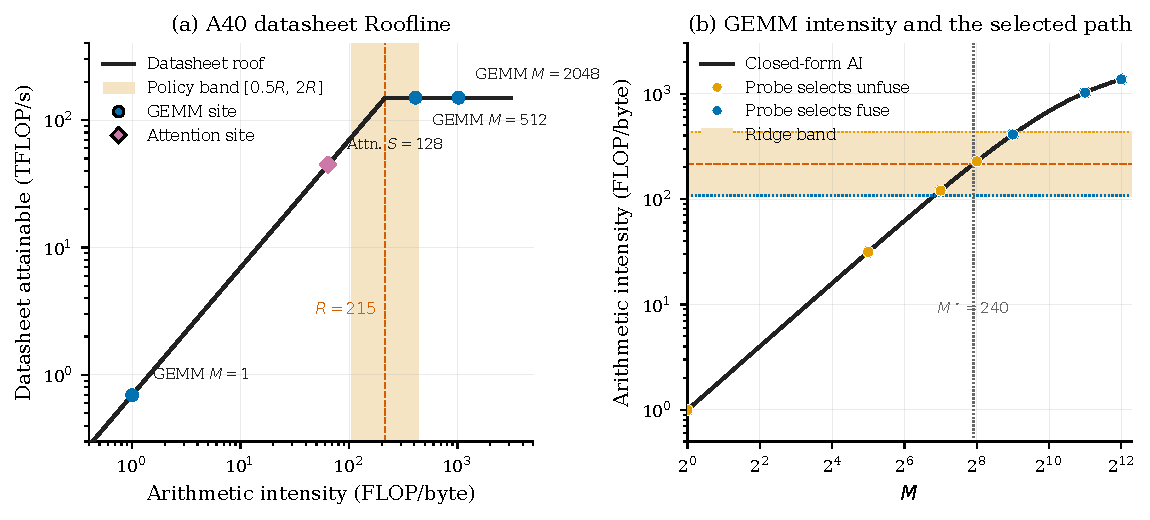
\includegraphics[width=\linewidth]{fig_roofline_gemm.pdf}
  \caption{Analytical intensity against the A40 datasheet, not a counter measurement.
  (a)~Datasheet roof, $149.7$~TFLOP/s over $696$~GB/s.
  Markers use \texttt{analytical\_ai} from the idle-GPU decision log and sit on the roof by construction.
  (b)~Closed form Eq.~\eqref{eq:square} for $N{=}K{=}4096$, FP16.
  Marker color is the wall-clock GEMM choice from the same log: unfuse at $M \in \{1,32,128,256\}$, fuse at $M \in \{512,2048,4096\}$.
  $M^{\star}{=}240$ is the datasheet balance point.}
  \label{fig:roofline}
\end{figure}

Fusing RMSNorm into that GEMM changes the byte count and does not change the GEMM FLOPs by much.
Unfused traffic reads $A$ and $B$, writes $C$, rereads $C$, reads the norm weight, and writes the normalized result.
Fused traffic drops the $C$ round trip.
For the square FP16 projection the saved fraction of unfused bytes is $2M/(d+4M)$ up to the norm weight in the denominator.
It grows with $M$: $0.05\%$ at $M{=}1$, $1.5\%$ at $M{=}32$, $10\%$ at $M{=}256$, $33\%$ at $M{=}2048$, and $40\%$ at $M{=}4096$.
The strict Roofline ratio of the unfused accounting over the fused one, using the A40 datasheet and no launch term, is $1.06\times$ at $M{=}128$ and $1.00\times$ for every shape with $M \ge 512$, because both accountings are then compute-limited.
Byte deletion at large $M$ does not move this model.
Section~\ref{sec:eval} shows that the PyTorch paths do not follow that prediction.

\subsection{Attention intensity}
\label{sec:attn-ai}

Let $Q,K,V$ have shape $[B,H,S,D]$.
An IO-aware prefill that keeps scores on chip and moves $Q$, $K$, $V$, and the output once has
\begin{equation}
  \AI = S / e,
  \label{eq:fa}
\end{equation}
so the head dimension cancels.
In FP16, $\AI{=}S/2$.
The bakeoff shapes therefore have analytical prefill intensities 64, 256, and 1024 at sequence lengths 128, 512, and 2048.
The A40 band labels those three sites memory-bound, ridge-region, and compute-bound.

Writing the scores changes the asymptote.
Charging three memory passes over the score tensor, intensity saturates at $4D/(3e)$ as $S$ grows.
For $D{=}128$ and FP16 that ceiling is $85.3$ FLOP/byte, below $0.5R$ on the H100 FP16 anchor ($R{=}295$).
Under this accounting, materializing scores keeps prefill memory-bound at every sequence length that fits the ceiling.
Fusion here is not a constant-factor saving on top of a compute-bound kernel.
It is the difference between a plan that can cross the ridge and a plan that cannot.
The bakeoff's eager attention baseline materializes scores.
Its SDPA baselines do not.
A speedup of SDPA over that eager baseline mixes the library algorithm with the epilogue choice, and the tables below keep those comparisons separate.

Decode fixes the query length at $S_q{=}1$ and grows the KV cache.
As the cache length grows,
\begin{equation}
  \AI \to \frac{2 H_q}{H_{kv}\, e}.
  \label{eq:decode}
\end{equation}
Multi-head attention in FP16 tends to $1$ FLOP/byte.
Grouped-query attention~\cite{Ainslie2023GQA} with $H_q/H_{kv}{=}8$ tends to $8$, which is still below $0.5R$ on every anchor in Table~\ref{tab:ridges}.
The two decode rows in the bakeoff are multi-head, $H{=}8$, $D{=}64$, and their logged intensities are $0.992$ and $1.000$.
A ``compute-bound attention'' label is a statement about IO-aware prefill.
It is the wrong label for decode.

The analytical selector never sets \texttt{materialize\_intermediate} on an attention plan.
ComputeMode on attention means large tiles and an epilogue that stays off the mainloop.
It does not mean a return to writing scores.

\subsection{Norms and ragged grouped GEMM}
\label{sec:moe}

RMSNorm, LayerNorm, softmax, residual add, and the other elementwise chains in the prototype are $O(1)$ FLOP/byte in FP16.
SCIC labels them memory-bound and emits MemMode only.
There is no compute-mode fission of a residual add.
Softmax over a materialized score matrix is charged $5$ FLOPs per score and $3$ memory passes, so its intensity is $5/(3e)$ and does not depend on $S$.

Grouped GEMM is where one layer holds more than one regime.
Expert $e$ computes $[t_e, H] \times [H, I]$.
Table~\ref{tab:moe} evaluates the closed form at $H{=}4096$, $I{=}14336$, FP16, against the H100 FP16 ridge, with inactive experts left unloaded except in the last row.
The skewed token histogram is the policy point: the $8$-token expert is memory-bound and the $1024$-token expert is compute-bound, while the token-weighted aggregate sits in the ridge band.
A single epilogue template for the whole layer is the wrong granularity.
The table is analytical.
The bakeoff does not time a mixture-of-experts layer~\cite{Shazeer2017MoE}.

\begin{table}[t]
  \centering
  \caption{Analytical grouped-GEMM intensity.
  $H{=}4096$, $I{=}14336$, FP16, H100 FP16 datasheet ridge.
  Agg., min, and max are intensities in FLOP/byte.
  Regimes use the occupied experts.
  The last row adds seven cold weight matrices and no extra FLOPs.}
  \label{tab:moe}
  \footnotesize
  \setlength{\tabcolsep}{4pt}
  \begin{tabular}{@{}lrrrrl@{}}
    \toprule
    Scenario & Tokens & Agg. & Min & Max & Regimes \\
    \midrule
    Decode, $8{\times}2$ & 16 & 2.00 & 2.00 & 2.00 & memory \\
    Balanced, $8{\times}256$ & 2048 & 237 & 237 & 237 & ridge \\
    Skewed, $1024{\ldots}8$ & 2040 & 236 & 7.98 & 775 & memory to compute \\
    Prefill, $8{\times}2048$ & 16384 & 1247 & 1247 & 1247 & compute \\
    One expert & 2048 & 1247 & 1247 & 1247 & compute \\
    All eight weights move & 2048 & 237 & 1247 & 1247 & aggregate ridge \\
    \bottomrule
  \end{tabular}
\end{table}

\subsection{Dual-plan rule}
\label{sec:selector}

Given a site report, the selector applies four rules.
\begin{enumerate}
\item Elementwise chains, reductions, softmax, and norms emit MemMode only.
\item A memory-bound site emits MemMode only.
A compute-bound site emits ComputeMode only.
\item A ridge-region site emits both plans.
The primary is MemMode when $\AI < R$ and ComputeMode otherwise.
\item Attention never materializes scores.
On a library-SDPA bakeoff the executable epilogue policy is \texttt{compile\_sdpa\_chain} in every regime, recorded as \texttt{always\_fuse}, including when the analytical primary is ComputeMode and \texttt{fuse\_epilogue} is false.
\end{enumerate}
For GEMM, the analytical binding is MemMode $\rightarrow$ \texttt{always\_fuse} and ComputeMode $\rightarrow$ \texttt{always\_unfuse}.
The ridge band still logs both plans.
The bakeoff times one executable path.

The GEMM path is then allowed to leave the analytical binding.
With calibration scope \texttt{all-gemm}, every MatMul+RMSNorm shape is probed for one warmup and three iterations.
The strictly faster median of \texttt{always\_fuse} and \texttt{always\_unfuse} is stored as \texttt{measured\_winner}.
Ties and missing times keep the analytical path.
The winner is a wall-clock comparison on the machine that runs the probe.
It is not DRAM arithmetic intensity.
The decision log marks that distinction as \texttt{WALLCLOCK\_CALIBRATION\_NOT\_DRAM\_AI}, and it records that GPU contention can flip the winner.
Attention is excluded from the probe.

Shape buckets for a plan cache are $1$, $2$--$8$, $9$--$32$, $33$--$128$, $129$--$512$, $513$--$2048$, $2049$--$8192$, and $8193+$.
The key is kind, dtype, machine, and bucket.
The bakeoff appends the shape label because that bucket would otherwise merge $M{=}256$ with $M{=}512$, which is the pair the measurement actually splits.

\section{Implementation}
\label{sec:impl}

The prototype is a Python package, \texttt{shapefuse} 0.3.1, with a classifier, a plan object, and a CUDA bakeoff harness.
\texttt{classify\_site} returns FLOPs, bytes, intensity, intensity over $R$, the three-way regime, and the strict Roofline resource.
The source of the intensity remains \texttt{analytical} until a measured intensity is supplied.
The A40 runs never supplied one.
\texttt{select\_plan} implements Section~\ref{sec:selector} and returns \texttt{kernel\_emitted=false}.

The harness times two subgraphs.

\paragraph{MatMul plus RMSNorm}
$N{=}K{=}4096$, FP16, at seven row counts from $M{=}1$ to $M{=}4096$.
The eager baseline and the unfuse path are the eager matrix product followed by RMSNorm.
The default compile path and the fuse path are \texttt{torch.compile} of that chain, timed separately, so their medians need not match.
Max-autotune is the same graph with \texttt{mode="max-autotune"} when the call returns.
The compiled graph is not inspected.
A compile-labelled row is evidence of a timed region, not evidence of a particular fusion pattern inside Inductor~\cite{Ansel2024PyTorch2}.

\paragraph{Attention plus RMSNorm}
The microbenchmark uses batch 1, eight heads, and head dimension 64.
Prefill lengths are 128, 512, and 2048.
Decode keeps a single query and uses cache lengths 128 and 2048.
The eager baseline materializes scores in PyTorch and then applies RMSNorm.
The SDPA baseline calls the library attention operator and then RMSNorm in one eager region.
\texttt{always\_fuse} compiles that SDPA-plus-norm chain.
\texttt{always\_unfuse} calls SDPA and times RMSNorm as a second region.
The SDPA kernel that the library selected was not logged.
The rows are PyTorch's library operator.
They are not a FlashAttention-3 kernel from this repository, and they are not a claim about which backend SDPA dispatched to.

\paragraph{Selected column}
\texttt{scic\_selected} copies the median of the baseline named by the decision.
On this run every GEMM decision is tagged measured wall-clock.
Every attention decision is tagged library SDPA and copies the fuse path.
Copying a median omits dispatch and plan-switch overhead.
The regular timing used three warmups and ten iterations.
The GEMM probe used one warmup and three.
\texttt{RUN\_NOTES.txt} records that all seven probe winners matched the faster of the two regular-timing baselines.

The run waited for two consecutive idle samples on the selected A40 before launching.
The script start reported $0\%$ utilization and $4$~MiB allocated.
A monitor that includes the benchmark peaked at $670$~MiB.
PyTorch was 2.5.1+cu121, CUDA 12.1, Python 3.10.12.
Dynamo's \texttt{cache\_size\_limit} was raised to $64$.
The run notes record no cache-limit warning.
Nsight Compute was not invoked.
An earlier A40 package did invoke \texttt{ncu} and failed with \texttt{ERR\_NVGPUCTRPERM} because GPU performance counters were restricted.
That failure is why achieved intensity is empty.

\section{Evaluation}
\label{sec:eval}

The claim we test is narrow.
On one idle A40, does the dual-plan binding pick a fast existing path, and where does that choice leave the datasheet label?
The answer is different for GEMM and for attention.
All latencies below are medians from the idle-GPU latency CSV.
Speedup is the eager median divided by the row median.
Values are rounded from the CSV.
Geometric means use the unrounded speedups.
Seventy-seven of seventy-seven latency rows completed.
Twelve decisions were logged.

\subsection{Shape dependence of a stock GEMM}
\label{sec:matmul}

Before any fusion comparison, a stock matrix product already changes throughput with $M$.
Table~\ref{tab:matmul} and Figure~\ref{fig:matmul} are the seven-shape A40 sweep in \texttt{paper/data/a40/bench\_gemm.csv} (\texttt{PARTIAL\_VENDOR\_MATMUL}, machine flag \texttt{A40\_FP16}).
The kernel is \texttt{pytorch\_matmul}.
No fused plan was timed.
From $M{=}1$ to $M{=}32$ the median stays near $0.07$--$0.08$~ms while the FLOP count grows by $32\times$, which is the launch-dominated end of a vendor GEMM.
At $M{=}4096$ the same call reaches $115.4$~TFLOP/s, $77.1\%$ of the A40 datasheet peak of $149.7$~TFLOP/s.
The curve supports shape dependence of achieved throughput.
It does not locate a measured ridge, and the Nsight byte column on every row is empty.

\begin{table}[t]
  \centering
  \caption{NVIDIA A40, stock \texttt{torch.matmul}, FP16, $N{=}K{=}4096$.
  Medians and TFLOP/s from \texttt{bench\_gemm.csv}.
  The band is the A40 datasheet band at the analytical intensity.
  \texttt{achieved\_ai} is empty on every row.}
  \label{tab:matmul}
  \small
  \begin{tabular}{@{}lrrrrl@{}}
    \toprule
    Label & $M$ & Median (ms) & TFLOP/s & $\AI$ & Band \\
    \midrule
    decode\_gemv & 1 & 0.0707 & 0.47 & 1.00 & memory \\
    micro\_batch & 4 & 0.0786 & 1.71 & 3.99 & memory \\
    decode\_batch32 & 32 & 0.0782 & 13.7 & 31.5 & memory \\
    near\_mstar & 344 & 0.142 & 81.3 & 295 & ridge \\
    ridge\_m512 & 512 & 0.179 & 96.1 & 410 & ridge \\
    prefill\_m2048 & 2048 & 0.659 & 104.3 & 1024 & compute \\
    square\_large & 4096 & 1.191 & 115.4 & 1365 & compute \\
    \bottomrule
  \end{tabular}
\end{table}

\begin{figure}[t]
  \centering
  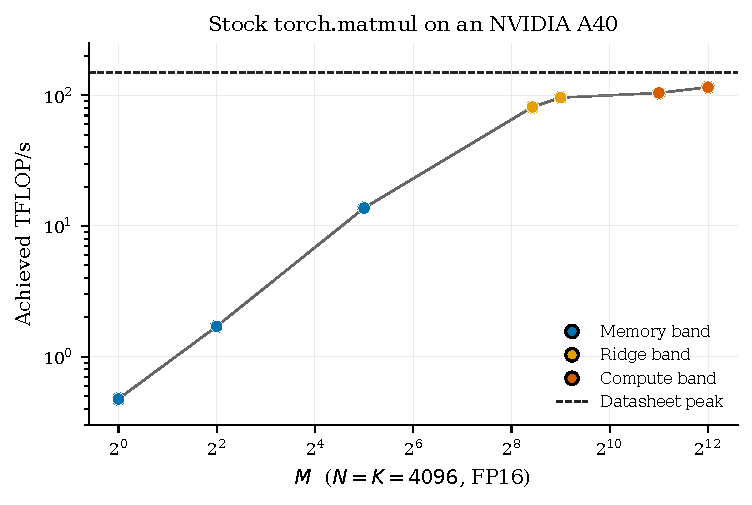
\includegraphics[width=0.78\linewidth]{fig_a40_torch_matmul_tflops.pdf}
  \caption{Achieved TFLOP/s of stock \texttt{torch.matmul} on the A40 sweep.
  The dashed line is the datasheet dense FP16 peak, $149.7$~TFLOP/s.
  Point color is the datasheet band of the analytical intensity.
  This is not a fused-plan comparison.}
  \label{fig:matmul}
\end{figure}

\subsection{GEMM: the probe matches the faster path}
\label{sec:gemm-eval}

Table~\ref{tab:gemm} is MatMul+RMSNorm on the idle bakeoff.
Figure~\ref{fig:gemm} plots the same speedups.
For $M \le 256$, \texttt{torch.compile} of the chain is slower than the eager chain: $0.763\times$ to $0.940\times$ versus eager.
For $M \ge 512$, the compiled chain is faster: $1.066\times$, $1.134\times$, and $1.187\times$.
The probe selects unfuse on the first four shapes and fuse on the last three.
Because the probe winner matched the faster regular-timing baseline on every GEMM shape, the copied SCIC median is the two-path oracle on this run.
The latency ratio of SCIC to $\min(\texttt{always\_fuse},\texttt{always\_unfuse})$ is $1$ on all seven rows (Figure~\ref{fig:oracle}).

\begin{table}[t]
  \centering
  \caption{MatMul+RMSNorm on the idle A40 (\texttt{bakeoff\_v4}).
  $N{=}K{=}4096$.
  Speedup is eager median divided by that path's median.
  ``Datasheet'' is the analytical binding before the probe.
  ``Selected'' is \texttt{measured\_winner}.
  SCIC copies the selected median.
  A separate \texttt{torch.compile} timing is within a few percent of the fuse column and is omitted here; it is the dashed line in Figure~\ref{fig:gemm}.}
  \label{tab:gemm}
  \footnotesize
  \setlength{\tabcolsep}{3.5pt}
  \begin{tabular}{@{}lrrllllrrr@{}}
    \toprule
    Shape & $M$ & $\AI$ & Band & Data. & Sel. & Eager & Fuse & Unfuse & SCIC \\
          &     &       &      &       &      & (ms)  & $\times$ & $\times$ & $\times$ \\
    \midrule
    decode & 1 & 1.00 & memory & fuse & unfuse & 0.088 & 0.763 & 0.994 & 0.994 \\
    decode & 32 & 31.5 & memory & fuse & unfuse & 0.100 & 0.840 & 0.999 & 0.999 \\
    ridge & 128 & 120 & ridge & fuse & unfuse & 0.104 & 0.864 & 0.999 & 0.999 \\
    ridge & 256 & 228 & ridge & unfuse & unfuse & 0.161 & 0.940 & 1.023 & 1.023 \\
    ridge & 512 & 410 & ridge & unfuse & fuse & 0.240 & 1.066 & 1.000 & 1.066 \\
    prefill & 2048 & 1024 & compute & unfuse & fuse & 0.874 & 1.134 & 1.000 & 1.134 \\
    prefill & 4096 & 1365 & compute & unfuse & fuse & 1.627 & 1.187 & 0.991 & 1.187 \\
    \bottomrule
  \end{tabular}
\end{table}

\begin{figure}[t]
  \centering
  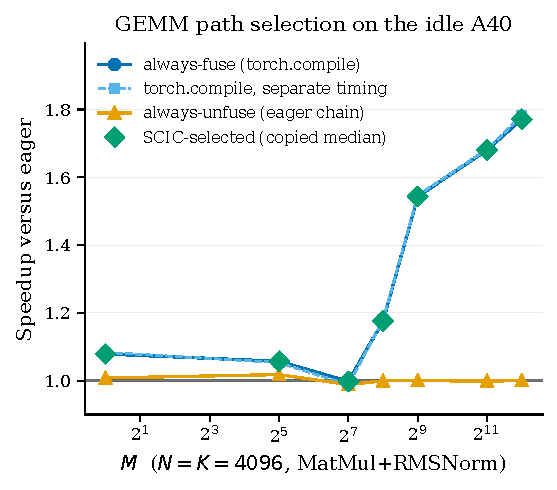
\includegraphics[width=0.92\linewidth]{fig_gemm_plan_speedup.pdf}
  \caption{Idle-A40 speedup of MatMul+RMSNorm versus the eager chain.
  The shaded interval is $M \in [256,512]$, where the measured winner changes.
  Green markers copy the faster of fuse and unfuse.
  \texttt{always\_fuse} and the separate \texttt{torch.compile} timing are two runs of the same compile recipe.}
  \label{fig:gemm}
\end{figure}

The datasheet primary agrees with that oracle at $M{=}256$ only.
On the memory side and at ridge $M{=}128$ it would have compiled a chain that is slower than eager.
On ridge $M{=}512$ and on both prefill shapes it would have refused the compiled chain that is faster than eager.
Following the primary yields a geometric mean of $0.921\times$ versus eager.
Following the probe yields $1.055\times$.
The ratio of those geometric means is $1.146\times$ on this shape set.
Always-fuse alone is $0.959\times$ and always-unfuse alone is $1.001\times$, because each static policy eats the shapes where it is the slower path.
Max-autotune is slower than eager on six of the seven shapes ($0.327\times$ at $M{=}1$ up to $0.954\times$ at $M{=}2048$) and $1.043\times$ at $M{=}4096$, still behind the fused median.

Two readings of this table should stay separate.
The first is empirical and is what we claim: for these two PyTorch paths, a three-iteration probe recovers the faster median, and the datasheet bit does not.
The second is about the cold-byte model, and it is negative.
At $M \ge 512$ that model gives a Roofline fusion speedup of $1.00\times$, because both the fused and the unfused byte counts are compute-limited, yet the compiled path is $1.07$--$1.19\times$ faster than eager.
The measured gain is therefore not the $C$-matrix round trip in Section~\ref{sec:gemm-ai}.
It may be a launch effect, a different GEMM schedule, or an epilogue overlap inside Inductor.
The graph was not inspected, so the paper does not assign the gain to one of those causes.
At $M \le 128$ the same model predicts a small byte win for fusion, and the compiled path is instead $0.763\times$ to $0.864\times$ versus eager.
MemMode's advice to fuse a memory-bound GEMM is the wrong direction for this binding.

The crossover itself sits where a dual plan is useful.
$M{=}256$ ($\AI{=}228$, just above $R{=}215$) still prefers unfuse.
$M{=}512$ ($\AI{=}410$, still below $2R{=}430$) prefers fuse.
Both shapes are ridge-region, so the analytical rule already emits both plans there.
The memory-side shapes are outside the band and would have received only MemMode.
Probing them is what avoids the compile regression.
Scope \texttt{all-gemm} is the setting that produced Table~\ref{tab:gemm}.

\subsection{Attention: the library policy is not the faster path}
\label{sec:attn-eval}

Table~\ref{tab:attn} and Figure~\ref{fig:attn} are the five attention shapes from the same run.
Every decision copies \texttt{always\_fuse}.
Against the score-materializing eager baseline, that choice is $1.187\times$, $0.920\times$, $5.588\times$, $1.122\times$, and $0.880\times$.
The geometric mean is $1.432\times$.
Most of the mean is the $S{=}2048$ prefill, where materializing scores costs about $1.07$~ms and every SDPA path costs about $0.16$--$0.19$~ms.
That gap is the library operator against a materialized score baseline.
It is not a comparison of epilogue policies.

\begin{table}[t]
  \centering
  \caption{Attention+RMSNorm on the idle A40.
  $B{=}1$, $H{=}8$, $D{=}64$.
  Eager materializes scores.
  SDPA, unfuse, and fuse all call library \texttt{scaled\_dot\_product\_attention}.
  Unfuse times RMSNorm as a second region.
  Fuse compiles SDPA and RMSNorm together.
  SCIC copies fuse on every row (\texttt{compile\_sdpa\_chain}).
  The SDPA kernel backend was not logged.}
  \label{tab:attn}
  \footnotesize
  \setlength{\tabcolsep}{3.5pt}
  \begin{tabular}{@{}llrrlrrrr@{}}
    \toprule
    Shape & Len. & $\AI$ & Band & Primary & Eager & SDPA & Unfuse & Fuse \\
          &      &       &      &         & (ms)  & $\times$ & $\times$ & $\times$ \\
    \midrule
    Prefill & $S{=}128$ & 64 & memory & Mem & 0.153 & 1.599 & 1.528 & 1.187 \\
    Prefill & $S{=}512$ & 256 & ridge & Comp & 0.157 & 1.507 & 1.456 & 0.920 \\
    Prefill & $S{=}2048$ & 1024 & compute & Comp & 1.072 & 6.865 & 5.584 & 5.588 \\
    Decode & $S_k{=}128$ & 0.992 & memory & Mem & 0.150 & 1.579 & 1.489 & 1.122 \\
    Decode & $S_k{=}2048$ & 1.000 & memory & Mem & 0.150 & 1.466 & 1.428 & 0.880 \\
    \bottomrule
  \end{tabular}
\end{table}

\begin{figure}[t]
  \centering
  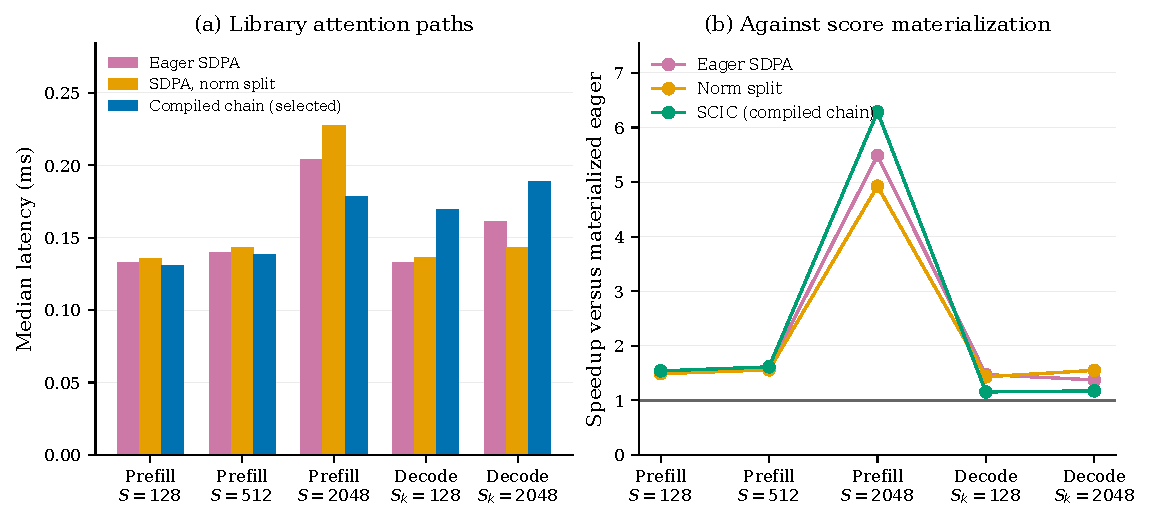
\includegraphics[width=\linewidth]{fig_attn_library_paths.pdf}
  \caption{Idle-A40 attention.
  (a)~Latency of the three library paths.
  The selected bar is the compiled chain.
  (b)~Speedup against the score-materializing eager baseline.
  The $S{=}2048$ peak is the library operator against materialized scores.
  Eager SDPA is the fastest bar or marker on every shape.}
  \label{fig:attn}
\end{figure}

Among the library paths the ranking is stable and unfavorable to the selected policy.
Eager SDPA is faster than the compiled chain on all five shapes.
The latency ratio of the compiled chain to eager SDPA runs from $1.23\times$ at $S{=}2048$ to $1.67\times$ at decode $S_k{=}2048$, with geometric mean $1.45\times$.
Splitting RMSNorm off SDPA is within $6\%$ of eager SDPA on four shapes and $1.23\times$ slower at $S{=}2048$.
Against the two-path choice the prototype is allowed to copy, fuse versus unfuse, the compiled chain is slower by $1.287\times$, $1.583\times$, $1.000\times$, $1.327\times$, and $1.622\times$.
The $S{=}2048$ pair differs by $0.13\,\mu\mathrm{s}$ ($0.07\%$), so that row is a tie for any decision this harness can justify.
The geometric mean of the five ratios is $1.344\times$.
Figure~\ref{fig:oracle} shows the contrast with GEMM: the GEMM bars sit on $1$, and four attention bars do not.

The analytical primary does not rescue the policy.
Prefill $S{=}512$ and $S{=}2048$ are ComputeMode, with \texttt{fuse\_epilogue} false, which would have split a further epilogue on a custom mainloop.
The executable rule overrides that bit and compiles the chain anyway, because an earlier busy-GPU archive had found the split slower when the analytical rule was followed literally.
On this idle GPU the override is the slower library placement.
Decode is MemMode, so the analytical primary and the library policy agree with each other, and both disagree with the faster timed path.
The data do not support a rule of the form ``fuse prefill, unfuse decode.''
Both decode shapes prefer the split, and the long prefill is a tie between split and compile, with eager SDPA ahead of both.

\begin{figure}[t]
  \centering
  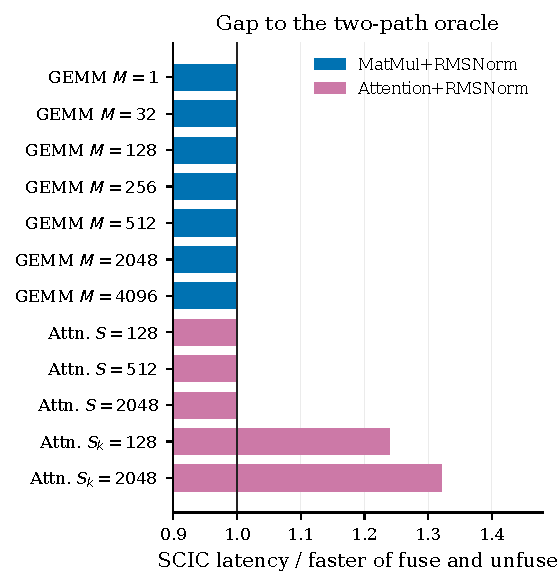
\includegraphics[width=0.86\linewidth]{fig_oracle_gap.pdf}
  \caption{Latency of the selected path divided by the faster of \texttt{always\_fuse} and \texttt{always\_unfuse}, using the regular ten-iteration medians.
  GEMM sits on $1$ because the wall-clock probe matched that minimum.
  Attention copies the compiled chain and meets the minimum only at $S{=}2048$, where the two medians differ by $0.07\%$.}
  \label{fig:oracle}
\end{figure}

\subsection{What the geometric means say}
\label{sec:summary}

Table~\ref{tab:summary} collects the shape-set geometric means.
On GEMM, the calibrated selector is the two-path oracle and is ahead of either static policy.
On attention, the selector is identical to always-fuse, the two-path oracle is the split-norm path, and eager SDPA is ahead of both.
We report these means as summaries of twelve microbenchmarks.
They are not a model-level speedup.

\begin{table}[t]
  \centering
  \caption{Geometric mean of per-shape speedups versus the eager baseline in the idle-GPU bakeoff.
  The eager attention baseline materializes scores, so the attention column mixes the library operator with the epilogue.
  Gap is the geometric mean of selected latency divided by the faster of fuse and unfuse, listed as GEMM / attention.
  A gap of $1$ means the selector matched that minimum.
  The gap cell is filled only for the selected policy.}
  \label{tab:summary}
  \small
  \setlength{\tabcolsep}{5pt}
  \begin{tabular}{@{}lccc@{}}
    \toprule
    Policy & GEMM ($n{=}7$) & Attention ($n{=}5$) & Gap \\
    \midrule
    Always fuse & 0.959 & 1.432 & --- \\
    Always unfuse & 1.001 & 1.925 & --- \\
    Datasheet primary & 0.921 & --- & --- \\
    Eager SDPA & --- & 2.073 & --- \\
    SCIC-selected & 1.055 & 1.432 & 1.000 / 1.344 \\
    \bottomrule
  \end{tabular}
\end{table}

The attention datasheet primary is not a single baseline name: the library override forces the executable path to fuse even when \texttt{fuse\_epilogue} is false, which is why that cell is left blank.
The GEMM datasheet row is well defined and is the quantity the probe improves on.

\subsection{What this run does not inherit from earlier archives}
\label{sec:archives}

Two earlier Docker archives used the same shape list on A40 cards that were not idle.
\texttt{paper/data/bakeoff/} recorded about $77$--$83\%$ utilization at startup and applied the analytical attention rule, which split RMSNorm off SDPA at prefill $S \in \{512,2048\}$.
\texttt{paper/data/bakeoff\_v2/} recorded $92\%$ utilization and $13490$~MiB already allocated on the selected GPU.
It introduced \texttt{compile\_sdpa\_chain} and still bound GEMM ComputeMode to \texttt{always\_unfuse}, with no wall-clock probe.
We do not compare milliseconds across those archives.
Load moves the medians, and the notes for the calibrated run say explicitly that contention can flip \texttt{measured\_winner}.
The decision difference is enough: the uncalibrated GEMM binding copies unfuse at $M \in \{256,512,2048,4096\}$, and the idle probe copies fuse at the last three of those four.
Quoted speedups in this section come only from the idle archive.

\section{Related work}
\label{sec:related}

\paragraph{Roofline}
The intensity--ridge picture is Williams et al.~\cite{Williams2009Roofline}.
Hierarchical and instruction-level extensions exist; we stay with the classical ridge because the quantity we need is a per-site label, and because we do not have the counters a hierarchical model would consume.
The datasheet substitution for $P$ and $B$ is a limitation of the present evidence, not a variant of the model.

\paragraph{IO-aware attention}
FlashAttention keeps the score tile on chip and changes both traffic and the kernel that implements attention~\cite{Dao2022FlashAttention,Dao2023FlashAttention2}.
FlashAttention-3 pushes that schedule onto Hopper asynchrony and low precision~\cite{Shah2024FlashAttention3}.
SCIC treats an IO-aware plan as one schedule that can be labeled, and a score-materializing plan as another.
The bakeoff calls PyTorch SDPA.
Which of those algorithms the library ran is not in the log.

\paragraph{Joint fusion}
ComFuse fuses matrix multiplication with memory-intensive epilogue subgraphs and lowers the result through a Stage-Stream execution model onto CUTLASS~\cite{Mu2026ComFuse,NVIDIACutlass}.
On its self-attention case, TorchInductor's FlashAttention library path outperforms the fused schedule, because the softmax stage does not hide behind the matrix product.
We read that case as evidence that one joint epilogue schedule is the wrong interface for attention.
We do not implement Stage-Stream, and we do not reproduce ComFuse's kernels.
RedFuser derives fused forms for cascaded reductions and generates GPU kernels, including attention-like patterns, on top of TVM~\cite{Tang2026RedFuser,Chen2018TVM}.
Neptune breaks selected reduction dependences and repairs them algebraically, recovering FlashAttention-like and FlashDecoding-like schedules from plain attention code~\cite{Zhao2026Neptune}.
Those systems emit kernels.
This paper stops at the regime label and at a choice among PyTorch paths.

\paragraph{Fusion granularity}
FuseFlow shows that full cross-expression fusion is not always the best granularity for sparse models on streaming dataflow hardware~\cite{Lacouture2026FuseFlow}.
The axis there is how large a fused region should be.
The axis here is which side of a dense-GPU ridge a concrete shape sits on.
The two questions are compatible and they are not the same experiment.

\paragraph{Compiler stacks}
TorchDynamo and TorchInductor are the \texttt{torch.compile} implementation we time~\cite{Ansel2024PyTorch2}.
Inductor lowers GPU graphs through Triton~\cite{Tillet2019Triton}.
Dynamic shapes expose symbolic dimensions.
They do not, in the bakeoff we ran, substitute for a measured choice between the compiled epilogue and the eager chain: the datasheet label and the faster path disagree on six of seven GEMM shapes.
We have not modified Inductor's fusion heuristics.
A prototype that fed the regime and the probed winner into those heuristics is future work.

\section{Limitations}
\label{sec:limits}

The ridge is a datasheet number.
\texttt{measured\_ridge\_flops\_per\_byte} is null.
A device-to-device copy probe in the earlier A40 package is archived as \texttt{ESTIMATE\_COPY\_NOT\_NSIGHT} and is not a substitute for that ridge.

Nsight DRAM bytes were not collected.
The attempt that did run \texttt{ncu} failed with \texttt{ERR\_NVGPUCTRPERM}.
A torch-profiler memory estimate on the stock matmul sweep equals the FP16 output matrix, so the implied intensity sticks at $K{=}4096$ and labels every shape compute-bound.
That estimate agrees with the analytical regime on two of the seven shapes.
The archive marks the rate as not valid SCIC accuracy.
We do not report it as classifier accuracy.
\texttt{quote\_as\_scic\_accuracy} remains false.

\texttt{scic\_selected} copies a baseline median.
Plan-switch cost on a length trace is unmeasured.
No MemMode or ComputeMode kernel was written, so the names in Section~\ref{sec:modes} have not been tested as tile shapes, register pressure, or shared-memory occupancy.
The $0.5R$/$2R$ band is a knob.
The softmax and RMSNorm flop constants are conventions.
The cold-byte model omits L2, masks, and paged KV.

The quoted bakeoff is one idle A40, one software stack, and one run of each shape.
A busy GPU can change the GEMM winner; the earlier archives are the evidence that the machine state matters, and they are not pooled with these medians.
Attention was not calibrated, and on this idle run the uncalibrated library policy is slower than eager SDPA.
Graphs were not inspected, so a compile speedup or regression is not yet a fusion recipe.
Fusion-proxy timings in the A40 package are marked as proxy timings rather than fusion speedups, and they are not results of this paper.
End-to-end tokens per second are not measured.

\section{Conclusion}
\label{sec:conclusion}

Shape decides which side of a Roofline ridge a GEMM or an attention site occupies, so a fusion planner needs a label that sees the shape and a scheduler that is allowed to keep two plans.
SCIC is that label, computed from closed-form traffic and a datasheet ridge.
The dual-plan rule is that scheduler, in miniature: MemMode, ComputeMode, or both inside the band.

Binding the plans to stock PyTorch paths changes what the label is allowed to mean.
On an idle A40, a few-shot wall-clock probe selects the faster of \texttt{torch.compile} and the eager MatMul+RMSNorm chain on all seven shapes, and the datasheet primary matches that choice once.
The same run's attention policy compiles library SDPA together with RMSNorm in every regime.
That policy beats a score-materializing baseline and loses to eager SDPA.
The honest reading is that intensity classification is the right compiler feature, and that a datasheet primary is not, by itself, the executable decision when the fused path is someone else's kernel.

The measurements that would tighten the label are still open: isolated DRAM bytes, a ridge measured on the card, kernels that actually implement the two tile regimes, and a serving trace that pays for switching plans.
Until those exist, the result to carry forward is the one in Table~\ref{tab:gemm} and Table~\ref{tab:attn}.
Classify the shape.
Keep both plans where the knee is uncertain.
Time the paths you can actually run.

\section*{Data availability}
The decision log, the latency log, and the run notes quoted above are \texttt{paper/data/bakeoff\_v4/}.
The stock matmul sweep is \texttt{paper/data/a40/}.
The figures are regenerated from those files by the plotting script in this paper directory.
No latency in Section~\ref{sec:eval} was typed in from a source other than those CSVs.

\section*{Declaration of competing interest}
The authors declare that they have no known competing financial interests or personal relationships that could have appeared to influence the work reported in this paper.

\bibliographystyle{elsarticle-num}
\bibliography{references}

\appendix
\section{Closed forms}
\label{app:formulas}

The intensities in Section~\ref{sec:method} are the functions in \texttt{shapefuse.intensity}.
Bytes are cold off-chip counts.
A multiply-add is two FLOPs.
Element size $e$ is in bytes.

\begin{center}
\small
\begin{tabular}{@{}lp{0.62\linewidth}@{}}
  \toprule
  Site & Arithmetic intensity \\
  \midrule
  GEMM & $2MNK / (MK e_A + KN e_B + MN e_C)$ \\
  Square projection & $2Md / ((d + 2M)\, e)$ \\
  Balance row $M(t)$ & $t\, e\, d / (2(d - t\, e))$ for $d > t\, e$ \\
  IO-aware prefill & $S / e$ \\
  Scores written, large $S$ & saturates at $4D / (3e)$ \\
  Softmax on scores & $5 / (3e)$ \\
  Decode, long cache & $2 H_q / (H_{kv}\, e)$ \\
  RMSNorm on $[M,K]$ & $4MK / ((2MK + K)\, e)$ \\
  Grouped expert & $2 t H I / ((tH)\, e_A + (HI)\, e_B + (tI)\, e_C)$ \\
  \bottomrule
\end{tabular}
\end{center}

The regime test is memory-bound if $\AI < 0.5R$, compute-bound if $\AI > 2R$, and ridge-region otherwise.
Roofline time, with no launch term, is $\max(\mathrm{FLOPs}/P,\ \mathrm{bytes}/B)$.

\section{Bakeoff path names}
\label{app:paths}

\begin{center}
\small
\begin{tabular}{@{}lp{0.72\linewidth}@{}}
  \toprule
  Name & What was timed \\
  \midrule
  eager & Eager MatMul then RMSNorm, or materialized attention then RMSNorm. \\
  compile & \texttt{torch.compile} of the fuse-attempt subgraph. The graph is not inspected. \\
  max-autotune & The same compile call with \texttt{mode="max-autotune"}, when it returns. \\
  sdpa & Eager SDPA, then RMSNorm. Attention rows only. \\
  always-fuse & The compile path. For attention this is the SDPA-plus-norm chain. \\
  always-unfuse & The eager GEMM chain, or SDPA and RMSNorm timed as two regions. \\
  scic-selected & A copy of the always-fuse or always-unfuse median named by the decision log. \\
  \bottomrule
\end{tabular}
\end{center}

\end{document}
